\documentclass[12pt]{article}
\usepackage{graphicx}
\usepackage{hyperref}
\usepackage{algorithm2e}
\graphicspath{ {./images/} }
\begin{document}

\section{Week 1 - Linear Regression}
\subsection{Introduction}
%Tell me about why you're interested in Machine learning
% What are some machine learning problems?

%//TODO add references to Coursera ML and Machine Learning for Humans book
Machine learning is all around us! Here are a couple examples that come to mind:

%//TODO: add overall outline and what we are intending to cover

It's why I don't have to sift through these emails in my inbox.

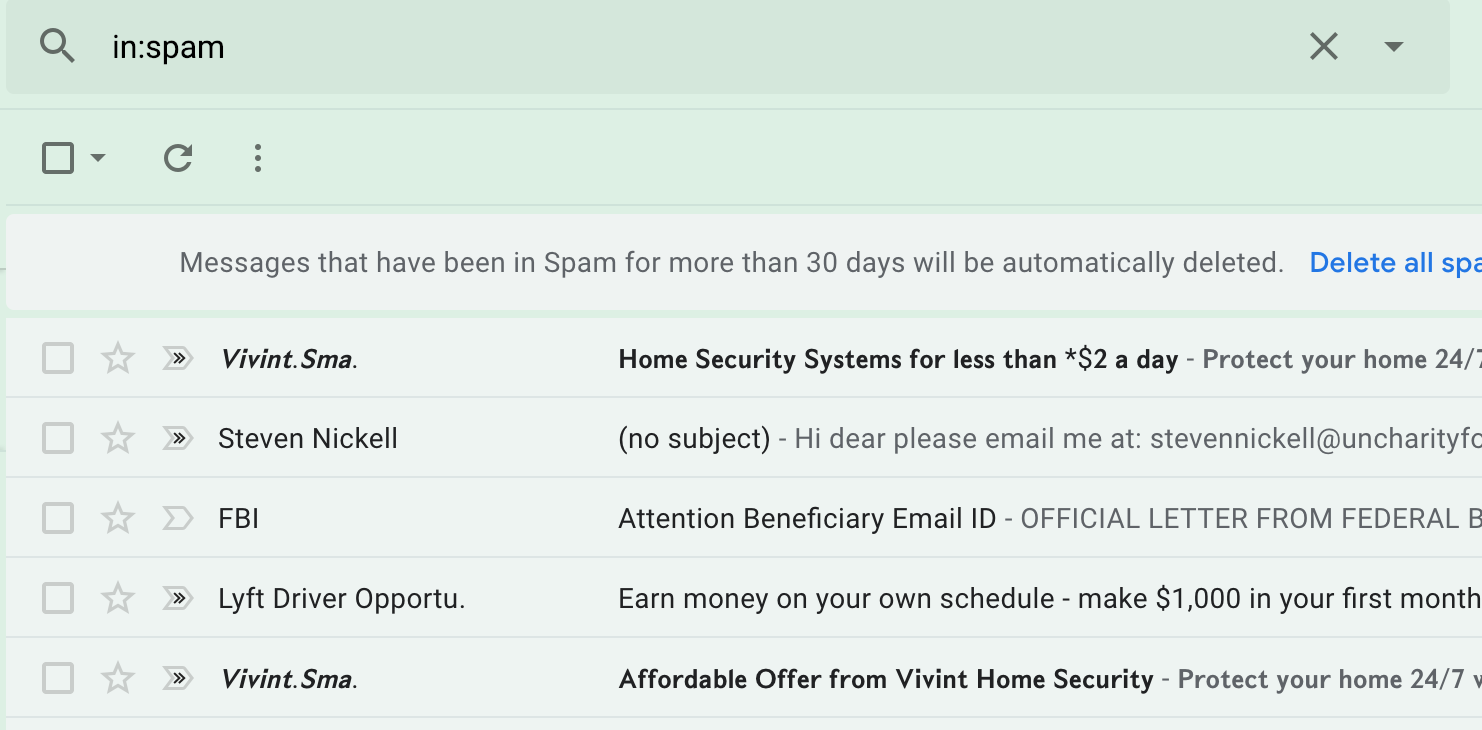
\includegraphics[width=0.75\textwidth]{spam}

It's why I can search my photos, by photos.

\begin{figure}[h]
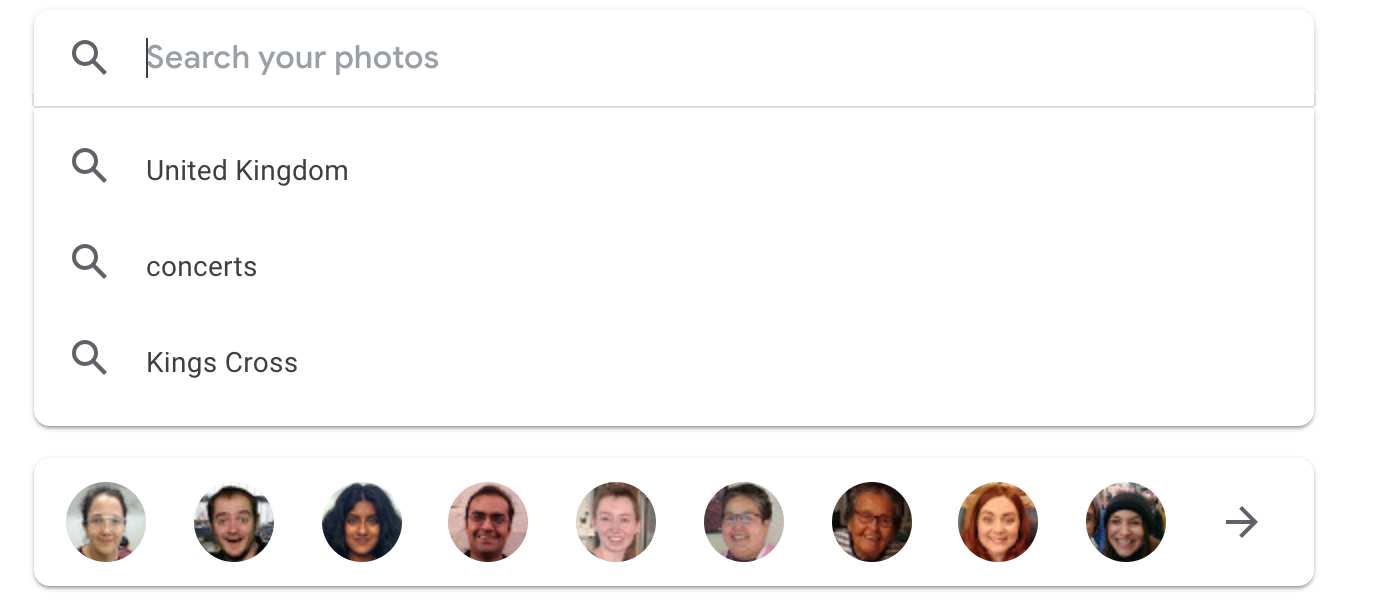
\includegraphics[width=0.75\textwidth]{photo-search}
\end{figure}


In this learning group we are going to learn a bit about \textit{Supervised Learning} in particular. If you're inspired to explore further, the Stanford Machine Learning \href{https://www.coursera.org/learn/machine-learning}{Stanford Machine Learning course} course on Coursera is a good place to start (indeed, you'll see that I took examples from it for the notes here when explaining regression and gradient descent). \href{https://medium.com/machine-learning-for-humans/why-machine-learning-matters-6164faf1df12}{Machine Learning for Humans} is also good.


\subsubsection{What is Machine Learning?}

According to wikipedia:
Machine learning (ML) is the scientific study of algorithms and statistical models that computer systems use to effectively perform a specific task without using explicit instructions, relying on patterns and inference instead.

Machine learning algorithms can learn to do a particular task without being explicitly programmed by building a mathematical model based on sample data, known as \textit{training data}. Then, that model can be applied to new data not previously used to build the model.

\subsubsection{What is an algorithm?}

An algorithm is often described as a set of steps to accomplish a particular task. I prefer to think about algorithms as means to solve computational problems. Computational problems are just well defined inputs and well defined desired outputs.

Here is a computational problem:

\textbf{Max of a set}

\textit{Input} A list of integers, unordered

\textit{Output} The largest integer in the list. 

An algorithm is simply a way to transform the input to the output. \\


Here's an algorithm for \textbf{Max of a set}:\\

\begin{algorithm}[H]
    \SetAlgoLined
    \KwData{\textit{inputList}, an unordered list }
    \KwResult{The largest integer in the list }
    Set $maxValueSoFar$ to the first value in the list \\
    
    \For{each item $i$ in \textit{inputList}}{
    
    \If{($v > maxValueSoFar$}{
    	$maxValueSoFar := v$
    }
    }
    \Return $maxValueSoFar$

    \caption{algorithm for \textbf{Max of a set}}
\end{algorithm}

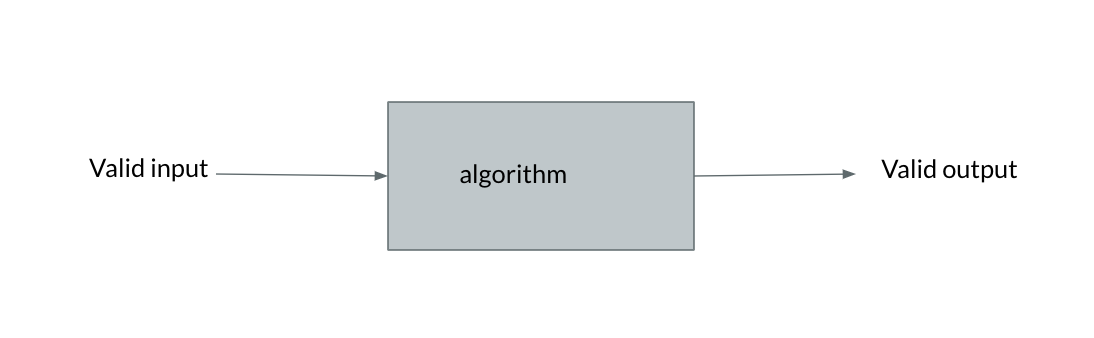
\includegraphics[width={0.75\textwidth}]{algo-abstract}

\textbf{Max of a set} should return the correct value each time, but for other computational problems we are very interested in measuring how accurate they are. Consider spam filters in real life. A spam filter that blocks 100 spam messages but lets through 1 spam message out of the 10,000 messages that have landed in your inbox is still a pretty good spam filter.

Let's linger a bit more on spam filters. The input would be an email message, and the output would be a classification (spam/not spam). The algorithm could be a set of steps. We could compose a series of regular expressions to the message that are based on previous messages that we know have turned out to be spam.

We could also train a model based on a dataset of emails and classifications, to learn patterns of what spam messages look like without explicitly writing spam identification rules. Then, we could use the model for new data that needs to be classified. That's the approach we're more interested in here, but both approaches are algorithms.

\subsubsection{What is a machine learning algorithm?}

Machine learning algorithms, just like any other algorithms, define some way to get from well defined inputs to some desired outputs. But

The ML Coursera course defines a \textit{Well Posed Machine Learning Problem}

A computer program is said to learn from experience $E$ with respect to some task $T$ and some performance measure $P$ 
if its performance on $T$, as measured by $P$ improves with experience $E$.

The important thing to note is that we are dealing with a machine learning algorithm if having more data to train our model improves our performance.

So, we can see that the rule based spam filtering approach wouldn't be a machine learning based approach because having more labelled data would not help us to classify spam any more accurately.

\subsubsection{Supervised Learning}

Here is an example of a supervised learning problem: 

Suppose we have a dataset of houses that have sold containing how much they have sold for, and the area of the property in square feet. 

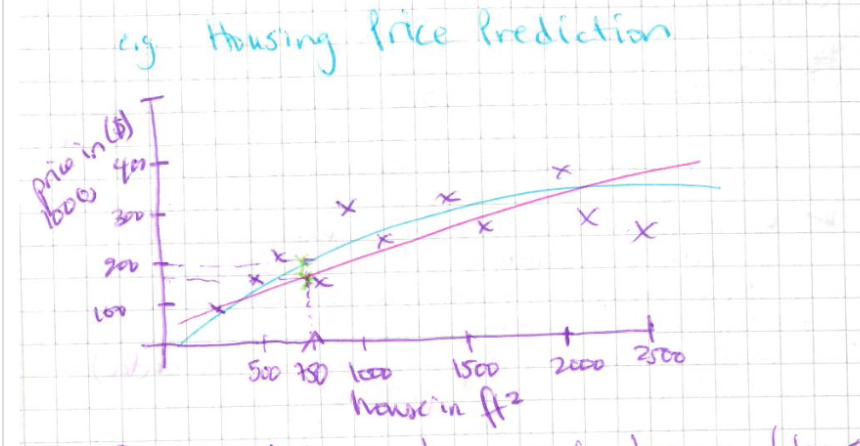
\includegraphics[width={\textwidth}]{housing-prices}

Then, we can use this data to build a model so that we can make a prediction like:

For this new 750 $ft^2$ property, how much will it sell for?

This is a \textit{Supervised Learning} problem because existing labelled data (with the right answers) to work with and to test how accurate our model is.

This is also a \textit{Linear Regression} problem because the prediction is a continuous valued output. 

Another example of a supervised learning problem would be:

Suppose we want to predict whether a tumour is benign or malignant, and we have a dataset that contains tumours, their size and whether they are benign or malignant.

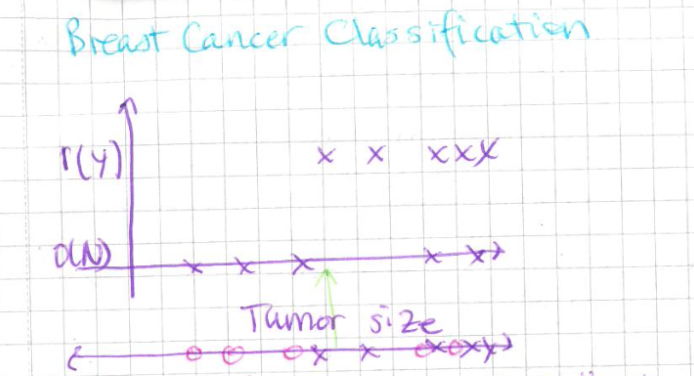
\includegraphics[width={\textwidth}]{tumour-size}

This would be a \textit{classification} problem, because the prediction is a discrete valued output (in this case, either benign or malignant). 

These might seem like toy examples so far. Cancer researchers will collect all sorts of data about tumours and patients that could all be useful in our model. But, we will aim to introduce concepts with a simplified view of the data to help our understanding, then move on to being able to use more features/data and more complicated techniques.

\subsubsection{Unsupervised Learning}

There is another area of Machine Learning, unsupervised learning that doesn't use labelled data to build a model. We won't cover unsupervised learning here, but let's introduce a couple unsupervised learning problems so that we'll get a feel for what these problems are like, and why they are different from supervised learning.

Here is an example of an unsupervised learning problem:


\includegraphics[width={\textwidth}]{google-news}

News aggregators will be able to cluster together news stories about the same topic even though that topic has not been seen before. No one has sat down and defined a \"Theresa May's second meaningful vote topic\", but a clustering algorithm will be able to find an underlying structure in news articles to be able to group them together, as seen above. 

Here is another example of an unsupervised learning problem:

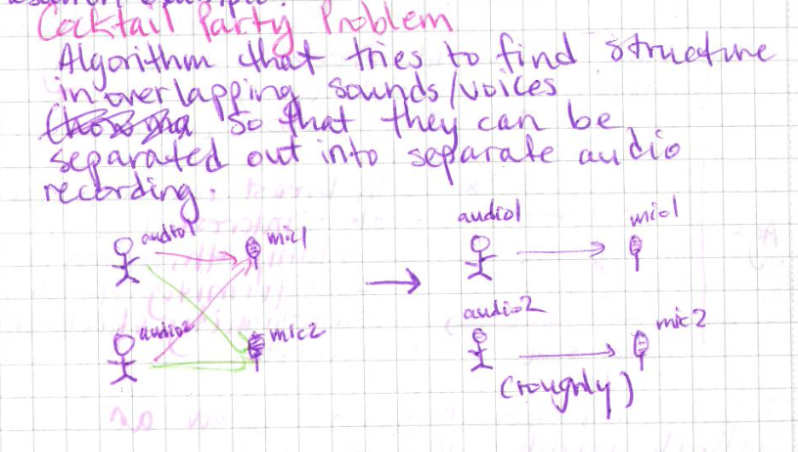
\includegraphics[width={0.75\textwidth}]{cocktail-party}

Given fixed mics in a room, and conversations happening around them, the mics will collect audio data for all of the conversations mixed together. If you want to be able to follow one of the conversations, an algorithm that identifies the underlying structure to be able to extract just the parts of the audio that belong to one conversation is an unsupervised learning problem.

\subsection{Linear Regression}
% do we want a different dataset ?
Let's move on to working through our first machine learning problem. We will first example a classic: house price prediction.

We will make use of the Ames house prices dataset. You can find out more about it \href{https://www.kaggle.com/c/house-prices-advanced-regression-techniques/data}{here}

The Ames dataset contains data about homes sold in Ames, Iowa between 2006 and 2010. This dataset has 79 features! But to start with, we are just going to use what seems like it might be the most important feature, the lot area to predict the house price.

Here is a sample from the dataset if we just extract the id, lot area, and selling price.
\begin{table}[htp]
\caption{Sample from a dataset of heights and weights}
\begin{center}
\begin{tabular}{|c|c|c|}
\hline
Id & LotArea & SellingPrice  \\ \hline
1143 & 9965.0 & 424870.0 \\
1105 & 2016.0 & 106000.0 \\
923 & 10237.0 & 169990.0 \\
499& 7800.0 & 130000.0 \\
1124 & 9405.0 & 118000.0 \\
\hline
\end{tabular}
\end{center}
\label{Sample from the Ames housing prices dataset.}
\end{table}%

%todo justify this
Let's plot lot area vs selling price for the training dataset.

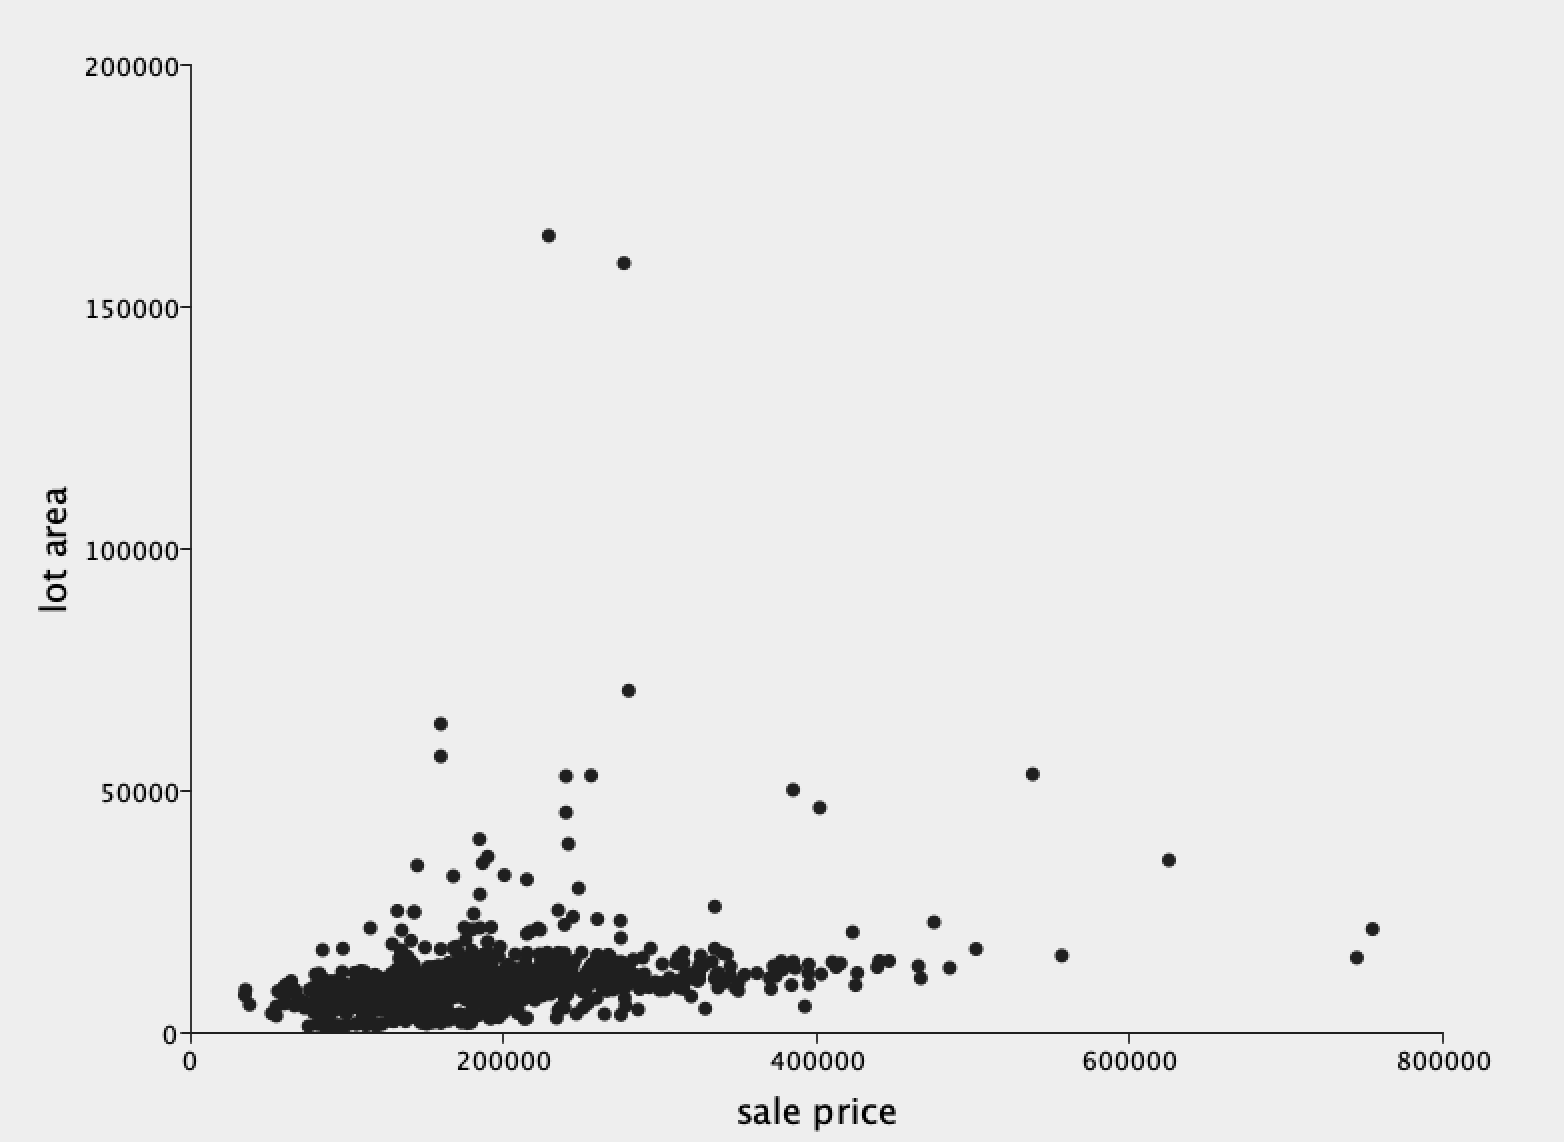
\includegraphics[width={\textwidth}]{ames-training-set}

It does seem reasonable to presume that lot area and selling price have a linear relationship.

Let's begin setting up our model.

\subsubsection{Training and Test Sets}

We can't use all of our data to build our model. We will portion our data into two parts:

\begin{enumerate}
\item Training data: data to help build our model
\item Test data: data to test the accuracy of our model, once it's already trained
\end{enumerate}

So now that we have a separate training set, here is some notation for how we will refer to the data:
\begin{table}[htp]
\caption{Sample from a dataset of lot size and selling price}
\begin{center}
\begin{tabular}{|c|c|}
\hline
notation & what is it \\ \hline
$m$ & the number of training examples \\
the $x$s e.g. $x_1$ & input variables/features \\
the $y$ & output variables/feature that we are trying to predict \\
$(x_1^i, y^i)$ & The $i$th training example  \\
\hline
\end{tabular}
\end{center}
\label{table:sample-table-notaton}
\end{table}%

So, in considering our housing price prediction problem, weight is $y$ and any other variables in the dataset that we might use to train our model are the $x$s.

\begin{table}[htp]
\caption{Sample from a dataset of lot size and house prices}
\begin{center}
\begin{tabular}{|c|c|c|}
\hline
$x_1$ & $x_2$ & $y$ \\ \hline
Id & LotArea & SellingPrice  \\ \hline
1143 & 9965.0 & 424870.0 \\
1105 & 2016.0 & 106000.0 \\
923 & 10237.0 & 169990.0 \\
499& 7800.0 & 130000.0 \\
1124 & 9405.0 & 118000.0 \\
\hline
\end{tabular}
\end{center}
\label{table:house-prices-sample-table-xs}
\end{table}%

Here, the \textit{learning algorithm} will, learning from our training data, produce a way to map from previously unseen $x$s to predicted $y$s.


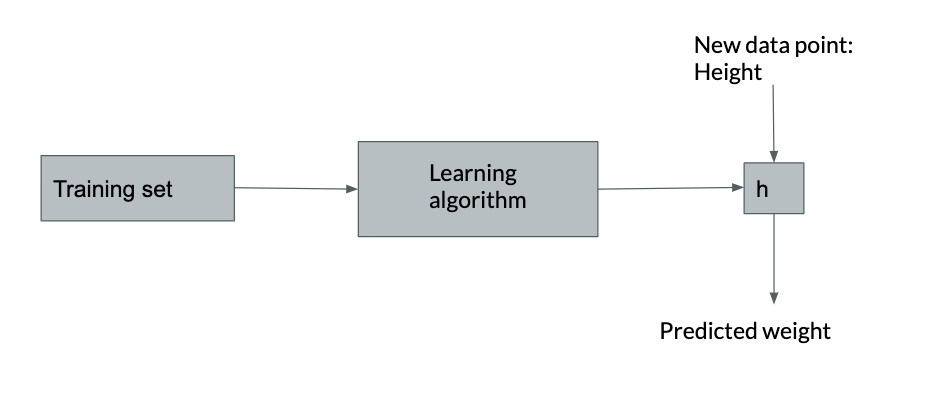
\includegraphics[width={\textwidth}]{the-model}

%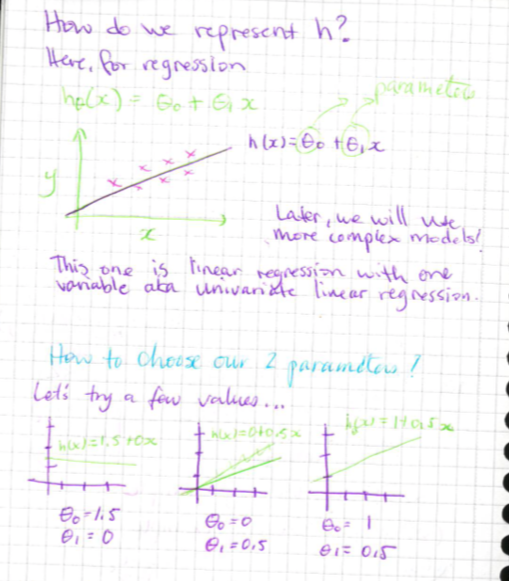
\includegraphics[width={\textwidth}]{regression-model}

So let's move onto finding $h$

Remember that we need a way to take previously unseen $x$s and predict $y$. Since our weight and height data seem to have a linear relationship, we will do this by fitting a line to our training data. This means that we're going to find \[h(x) = \theta_0 + \theta_1x\] such that when we evaluate some $h(x^{(i)})$, it will be as close to $y^{(i)}$ as possible.

We need a way, more formally, to say how well our $h(x)$ fits our training data. We will compare the $y$ predicted by $h(x)$ for each data point, and sum up the differences with the following function:

\[J(\theta_0, \theta_1) = \frac{1}{2m} \sum^m_{i=1}(h_\theta(x^{(i)}) - y^{(i)})^2\]

(Recall: $h_\theta(x) = \theta_0 + \theta_1x$)

In short, here is our model:

\textbf{Hypothesis}: $h_\theta(x) = \theta_0 + \theta_1x$ (we think that a line will fit our data)

\textbf{Parameters}: $\theta_0$, $\theta_1$

\textbf{Cost function}: \[J(\theta_0, \theta_1) = \frac{1}{2m} \sum^m_{i=1}(h_\theta(x^{(i)}) - y^{(i)})^2\]

\textbf{Goal}: minimise $J(\theta_0, \theta_1)$. Once we have $\theta_0$, $\theta_1$, we can plug them into our hypothesis and make predictions!

\end{document}